\documentclass{abnt}

\usepackage[utf8]{inputenc}
\usepackage[brazil]{babel}
\usepackage[num]{abntcite}

\usepackage{listings}
\usepackage{color}
\usepackage{float}
\usepackage{graphicx,url}

\setcounter{secnumdepth}{5}

%%%%%%%%%%%%%%%%%%%%%%%%%%%%%%%%%%%%%%%%%%%%%
% INFORMACOES SOBRE OS AUTORES, TITULO, ...
\autor {Bruno Nocera Zanette}
\titulo {Conversão de algoritmos de processamento de dados meteorológicos de C para CUDA}
\instituicao{Universidade Federal do Paraná}
%\orientador{Prof. Fabiano Silva}
\data{Curitiba, Abril de 2013}
\comentario{Trabalho de conclusão de curso de Bacharelado em Ciência da Computação.
\\
\\Orientador: Prof. Fabiano Silva}
%%%%%%%%%%%%%%%%%%%%%%%%%%%%%%%%%%%%%%%%%%%%%

%%%%%%%%%%%%%%%%%%%%%%%%%%%%%%%%%%%%%%%%%%%%%
%Definicao do estilo dos codigos
%Baseado em:
%http://en.wikibooks.org/wiki/LaTeX/Source_Code_Listings

\definecolor{mygray}{rgb}{0.5,0.5,0.5}

\renewcommand{\lstlistingname}{Código-Fonte}

\lstdefinestyle{code_style}{
language=C,
breaklines=true,
frame=tb,
commentstyle=\color{mygray},
basicstyle=\footnotesize,
numbers=left,
numbersep=5pt,
numberstyle=\color{mygray},
tabsize=2,
showtabs=false
}
%%%%%%%%%%%%%%%%%%%%%%%%%%%%%%%%%%%%%%%%%%%%%

\begin{document}

\capa

\folhaderosto

\sumario

%\chapter*{Lista de Abreviaturas e Siglas}
\begin{itemize}
\item[\textbf{ABIC}] - Associação Brasileira de Café
\end{itemize}
\listadefiguras

\chapter*{Resumo}

Neste trabalho farei um estudo de caso do processo de conversão de um algoritmo de processamento de dados da linguagem C para CUDA, com o intuito de mostrar que a relação custo e benefício dessa tarefa pode ser muito boa. Além disso o trabalho tem como um segundo objetivo criar um modelo de código para que este possa ser usado como suporte para a conversão de novos algoritmos.
\chapter{Introdução}

A meteorologia é uma das áreas que mais exige poder computacional para alcançar seus objetivos. A previsão meteorológica é o exemplo mais claro disso. Tal tarefa necessita de supercomputadores, como por exemplo o novo supercomputador Cray XT-6 adquirido pelo CPTEC/INPE considerado um dos 50 mais rápidos do mundo, e equipes especializadas em otimizar o código-fonte dos programas para ser capaz de alcançar bons resultados. Isso acontece porque para alcançar tamanha precisão é necessário que os dados utilizados como base tenham uma resolução igualmente boa. Porém isso faz com que a quantidade de dados a ser processado seja muito maior, e assim elevando o tempo de execução.

Entretanto, o campo da meteorologia não se resume apenas a previsão atmosférica. Existem muitos laboratórios espalhados pelo mundo que realizam pesquisas igualmente importantes e que enfrentam problemas similares aos já citados. A diferença é que por um lado tais pesquisas não necessitam de dados com tanta precisão, mas que por outro não possuem tanto investimento para equipamentos melhores. Outra grande diferença é que nessas pesquisas são os próprios pesquisadores, normalmente da área de física ou engenharia, que escrevem e executam os programas. Uma consequência disso é que os programas normalmente não são escritos da forma mais eficaz, fazendo com que algoritmos simples tenham um tempo elevado de execução, e assim desperdiçando o hardware disponível.

Nesse trabalho será estudado métodos para otimizar algoritmos de processamento e análise de dados atmosféricos com base em técnicas de programação paralela, visando auxiliar programadores com pouco experiência a reduzir o tempo de execução de algoritmos. Nos próximos capítulos será detalhado a organização dos dados utilizados, as técnicas utilizadas e os resultados obtidos.





\chapter{Algoritmos atmosféricos}\label{cap:algs_atmosfericos}

O objetivo desses algoritmos é processar uma base de dados, com base em conceitos estatísticos, de tal forma a gerar novas informações que possam ser usadas em pesquisas e estudos relacionados à área atmosférica. Grande parte desses algoritmos se baseiam no processamento de uma única série de dados e calculam a informação para apenas essa série, da mesma forma como é feito quando calcula-se a média de uma série de valores. Na verdade, muito desses algoritmos também podem serem usados em outras áreas com a diferença do tipo do dado de entrada usado e alguns pequenos ajustes. Posteriormente esses algoritmos são aplicados para um conjunto de séries relacionadas a diferentes locais da área a ser estudada, como será descrito nos próximos capítulos. Um fato importante a se notar é de que, normalmente, o processamento de cada uma das séries é independente uma das outras. 

Para exemplificar usaremos os algoritmos Filtro de Lanczos e Teste de Monte Carlo, pois cada um possui caraterísticas próprias que fazem com que a execução dos mesmos possa ser muito demorada quando executados sequencialmente.

\section{Filtro de Lanczos}

O algoritmo Filtro de Lanczos, descrito por \cite{Duchon:1979}, é utilizado, entre outras coisas, para filtrar variações temporais de dados atmosféricos diários. O problema consiste em calcular resultados para um certo vetor de dados, multiplicando-se um vetor de constantes de tamanho menor, $WT$, previamente calculado, com um pedaço da serie de dados, e armazenando o resultado numa nova série de dados, na posição central, como descrito na fórmula a seguir e exemplificado na figura \ref{fig:representacao_calculos_lanczos}.

\[
Para \; (t=1\;,\;NT): \;
Res[t + \lfloor \frac{K}{2} \rfloor ]=\sum _{i=1} ^{K} ( WT[i] \times Dados[t+i-1] )
\]

%%%%%%%%%%%%%%%%%%%%%%%%%%%%%%%%%%%%%%%%%%%%%%%%%%%%%%%%%%
% FIGURA
\begin{figure}[H]
\centering
\includegraphics[width=0.4\textwidth]{Imagens/representacao_calculos_lanczos/representacao_calculos_lanczos.png}
\caption{Representação abstrata dos cálculos para K=5}
\label{fig:representacao_calculos_lanczos}
\end{figure}
%%%%%%%%%%%%%%%%%%%%%%%%%%%%%%%%%%%%%%%%%%%%%%%%%%%%%%%%%%

Para cada resultado produzido por esse algoritmo são necessárias $K$ somas e multiplicações, onde $K$ é o número de pesos usados, definidos por \cite{Duchon:1979}. Uma vez que os dados de entrada usados para esses algoritmos possuem centenas de séries de centenas de valores cada uma, como será descrito mais a frente, o tempo de execução desse algoritmo, mesmo sendo uma função sequencial relativamente simples, tende a ser muito grande.

\section{Teste de Monte Carlo}

O teste de Monte Carlo é utilizado, dentro da área de estudos atmosféricos, para calcular a significância entre duas séries distintas. Esse algoritmo faz parte de uma classe de algoritmos que utilizam o método de Monte Carlo, o qual se baseia na observação de valores aleatórios e o uso dessa amostra para o cálculo da função de interesse.

O algoritmo a ser estudado nesse trabalho foi retirado de \cite{Joao:2010} e é dado pelos seguintes passos, sendo $n_{e}$ o número de experimentos do teste de Monte Carlo:

\begin{enumerate}
\item  é calculado o coeficiente de correlação entre as séries A e B. Por simplicidade, a correlação entre essas duas séries será chamada de correlação original;\footnote{O cálculo da correlação é linear, e exige aproximadamente $NT*10$ operações, onde $NT$ é a quantidade de valores em cada série}

\item  a séria A sofre permutação entre seus membros, a fim de se formar uma nova série;

\item  é calculado o coeficiente de correlação entre esta nova série e a série B;

\item  compara-se o novo coeficiente de correlação com o anterior;

\item  repete-se os passos 2,3 e 4, $n_{e}$ vezes;

\item  chamando de $cor_{m}$ o número de vezes em que o novo coeficiente de correlação foi maior do que o original, o nível de significância é definido como a razão entre $cor_{m}$ e $n_{e}$;
\end{enumerate}

O tempo de execução desse algoritmo pode ser bastante elevado dependendo do valor $n_{e}$, pois o mesmo define a quantidade de novas séries a serem geradas e de cálculos de novos coeficientes de correlação. Sabendo-se que essas séries podem conter centenas de valores, a quantidade de acessos a memória necessários para escrever e ler todos esses valores é muito grande, elevando o tempo de execução consideravelmente.
\chapter{Organização dos dados}

Os dados utilizados como entrada para esses algoritmos são baseados em séries temporais de valores que representam o comportamento de alguma variável atmosférica, tal como quantidade de chuva e temperatura do ar, num local específico em vários momentos do tempo. Essas informações podem ser obtidas por satélites, balões atmosféricos, estações meteorológicas, entre outros, e normalmente são medidas uma ou mais vezes por dia. A partir da obtenção dessas séries de dados em diversos locais espelhados por uma determinada área, ou até mesmo no globo terrestre inteiro, são feitas verificações para a validação desses valores obtidos e executado métodos para a dedução dos valores referentes a localidades onde não é possível fazer a medição, como por exemplo no meio dos oceanos. Enfim é criado uma grade que divide igualmente a área de interesse em pequenas quadrículas, de tal forma que cada uma dessas áreas seja representada por apenas uma série de dados, e de que a visualização como um todo dessas várias séries represente o comportamento da variável em questão na área total. 

Em geral a utilização de apenas uma série de dados para cada uma dessas áreas pode gerar muitas informações equivocadas, uma vez que o comportamento dessas variáveis atmosféricas podem variar bruscamente dentro de cada uma dessas regiões. Por isso há a necessidade de que o tamanho dessas regiões seja o menor possível. Entretanto isso faz com que haja muito mais séries para a mesma área de interesse, o que numa escala global faz com que o número de quadrículas cresça bruscamente.

Existem diversas instituições que fornecem livremente esses dados ao público, como o National Oceanic \& Atmospheric Administration e a NASA \cite{NASA} dos Estados Unidos da América,e o Met Office Hadley Centre \cite{MOHC} da Inglaterra. São dados como esses que servem como base para estudos sobre mudanças climáticas.

\section{Estrutura de dados}

A estrutura de dados usada para armazenar essas informações é uma matriz tridimensional (X,Y,T) na qual os eixos X e Y se referem a posição espacial e o eixo T ao tempo, e cada um desses eixos possui uma quantidade fixa de valores, respectivamente NX, NY e NT. Essa estrutura é armazenada de forma sequencial variando primeiramente os eixos X e Y e por fim o eixo T, ou seja, os valores do eixo T para cada ponto (X,Y) ficam separados.

\section{Tamanho dos dados}

Um dos principais desafios enfrentados no uso desses dados é o tamanho dos arquivos necessários para armazenar toda a informação, que pode ser calculado multiplicando-se o número total de quadrículas (NX * NY) pelo tamanho de cada uma das séries de dados (NT). Por exemplo, para armazenar as informações referentes a 1 ano de valores diários, para uma grade global de 360 por 180 quadrículas são necessários 94608000 bytes (NT=365 x [NX=180 * NY=360] x 4 bytes), ou aproximadamente 90MB. Pode não parecer muito mas, sabendo-se que cada uma dessas quadrículas abrange uma área de aproximadamente 110Km$^2$ e são as informações de apenas 1 ano, percebe-se que para um período de dados um pouco maior ou para quadrículas com uma área um pouco menor esse valor pode chegar facilmente nas casa dos GigaBytes. Prova disso é que, para esse mesmo exemplo citado, caso fosse um período de 50 anos seriam necessários 4.4GBs.

%%%%%%%%%%%%%%%%%%%%%%%%%%%%%%%%%%%%%%%%%%%%%%%%%%%%%%%%%%
% FIGURA
\begin{figure}[H]
\centering
\includegraphics[width=1.0\textwidth]{Imagens/tamanho_dados/serie_tam_dados.png}
\caption{Gráfico do tamanho dos arquivos de dados}
\label{fig:grafico_tamanho_dados}
\end{figure}
%%%%%%%%%%%%%%%%%%%%%%%%%%%%%%%%%%%%%%%%%%%%%%%%%%%%%%%%%%
\chapter{Implementação paralela dos algoritmos}

Como descrito anteriormente, o processamento de cada quadrícula de dados é feita de forma independente uma da outra, fazendo com que a implementação paralela desses algoritmos seja algo natural a se fazer. Entretanto, existem alguns problemas a serem enfrentados para o sucesso dessa tarefa, especialmente ao usar a plataforma CUDA.

Nesse capítulo serão analisadas as principais etapas e dificuldades das implementações paralela em OpenMP \cite{openmp_guide} e CUDA \cite{cuda_guide} dos algoritmos Filtro de Lanczos e Teste de Monte Carlo, apresentados no capítulo \ref{cap:algs_atmosfericos}.

\section{Implementação em OpenMP}

A maior vantagem em se usar as bibliotecas OpenMP \cite{openmp_guide} para implementar soluções paralelas desses algoritmos é a facilidade. Isso se dá primeiramente pelo fato de que não é necessário um tratamento especial da memória, diferente da implementação em CUDA, e principalmente por se tratar da adição de pouquíssimas linhas de código com a função de apenas especificar como a função em questão deve ser paralelizada.

Esses fatores são especialmente importantes no caso dos algoritmos estudados pois o fato de não haver mudanças mais profundas no código há uma maior confiança nos resultados obtidos. Além disso, o código é capaz de rodar em qualquer processador e não é necessário a  reconfiguração de nenhum parâmetro para que a execução em máquinas diferentes seja a melhor possível, pois a configuração do número de threads já é feita durante a execução. Isso faz com que seja muito fácil o uso dessa solução por parte dos pesquisadores em qualquer máquina.

Porém, como será descrito mais a frente, essa solução possui uma escalabilidade muito pequena, e em alguns casos o tempo de execução pode ser até maior do que a implementação sequencial. Por estas razões essa implementação será usada apenas como referência.

\section{Implementação em CUDA}

Diferente da solução com base em OpenMP, a implementação em CUDA \cite{cuda_guide} possui uma grande escalabilidade e reduziu significantemente o tempo de execução em todos os testes realizados. Porém, a sua implementação necessita de muito mais cuidados, além de uma placa-de-vídeo que suporte a tecnologia CUDA.

CUDA é uma arquitetura criada pela empresa NVidia que utiliza placas-de-vídeo para executar algoritmos em paralelo, utilizando as centenas de núcleos de processamento presentes nessas placas, também chamadas de GPUs. Dentro do contexto CUDA essa placa é chamada de device e a máquina em que esse device está acoplado é chamada de host.

Outros fatores importantes a se notar é que essas placas possuem uma memória própria e que a cópia da memória entre o host e o device não é feita automaticamente a quantidade, além de que a quantidade dessa memória existente é limitada e não há a possibilidade de expansão. São esses fatores que fazem com que a implementação seja mais difícil, especialmente no caso dos algoritmos estudados os quais, como já explicado, necessitam de uma grande quantidade de memória.

\subsection{Proposta de solução}\label{cap:proposta_solucao}

Uma solução para possibilitar o uso desses algoritmos em qualquer plataforma CUDA, independente do tanto de memória disponível, é processar esses dados em ciclos de processamento, ou seja, processar apenas uma parte dos dados de entrada a cada ciclo. Porém os mesmos são originalmente organizados de forma que os valores dos eixos X e Y fiquem juntos, fazendo com que os valores de uma quadrícula no eixo do tempo fiquem separados, o oposto do que seria o ideal. Isso não é nenhum obstáculo quando pensamos numa execução sequencial do algoritmo, onde a quantidade e facilidade de acesso à memória é maior, mas impossibilita a ideia de ciclos de processamentos, pois impede que os mesmos sejam repartidos.

%%%%%%%%%%%%%%%%%%%%%%%%%%%%%%%%%%%%%%%%%%%%%%%%%%%%%%%%%%
% FIGURA
\begin{figure}[H]
\centering
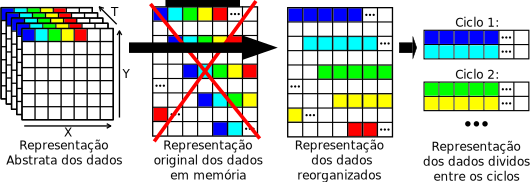
\includegraphics[width=0.8\textwidth]{Imagens/organizacao_dados/organizacao_dados.png}
\caption{Organização dos dados}
\label{fig:organizacao_dados_2}
\end{figure}
%%%%%%%%%%%%%%%%%%%%%%%%%%%%%%%%%%%%%%%%%%%%%%%%%%%%%%%%%%

Para contornar isso foi utilizado uma função de leitura que armazena os dados na memória do Host de forma que a série de tempo de cada quadrícula seja contínua, como demonstrado na figura (\ref{fig:organizacao_dados_2}), assim sendo possível copiar pedaços separados desse dado para o device. Além disso, ao invés da estrutura de matriz, foi usado a estrutura de um vetor comum para armazenar esses valores e funções auxiliares para calcular a posição na memória em que se inicia os dados de cada quadrícula. Essa decisão ainda facilita a cópia de dados entre a memória do Host e do Device.

\subsection{Implementação da solução}\label{cap:implementacao_solucao}

Em teoria essa tarefa seria a mais difícil do processo de implementação do algoritmo em CUDA, porém foi a que menos precisou de ajustes. Na função que implementa o algoritmo em si as únicas alterações necessárias foram remover o loop de incremento das quadrículas a serem processadas, necessário na versão sequencial, e adicionar o cálculo que defini qual quadrícula cada um dos núcleos de processamento do device será responsável por processar. Essas alterações estão detalhadas na figura \ref{fig:comparacao_codigo_padrao}, juntamente com as necessárias para implementar a solução em OpenMP.

%%%%%%%%%%%%%%%%%%%%%%%%%%%%%%%%%%%%%%%%%%%%%%%%%%%%%%%%%%
% FIGURA
\begin{figure}[H]
\centering
\includegraphics[width=0.7\textwidth]{Imagens/comparacao_codigo/comparacao_codigo_padrao.png}
\caption{Comparação da função que implementa o algoritmo}
\label{fig:comparacao_codigo_padrao}
\end{figure}
%%%%%%%%%%%%%%%%%%%%%%%%%%%%%%%%%%%%%%%%%%%%%%%%%%%%%%%%%%

Foi a função \texttt{Main} do código em C que sofreu as maiores mudanças, como pode ser visto na figura \ref{fig:comparacao_codigo_main}. Porém, grande parte dessas alterações foram apenas para adicionar as premissas básicas de todo programa, como alocação e inicialização de memória, no contexto do CUDA. As outras modificações foram a adição das funções de cópia de memória entre Host e Device e um loop para controlar os ciclos.

Esses ciclos foram pensados para o caso da memória total necessária para armazenar os dados de entrada e saída for maior do que o total de memória disponível no device. Para que esse método funcione, além da organização dos dados previamente descrita, foi criado um pequeno algoritmo para dividir igualmente o processamento entre os vários ciclos. Dentro de cada um desses ciclos as seguinte ações são executadas, em ordem:

\begin{enumerate}
\item Cálculo da posição de início da cópia dos dados de entrada;
\item Cópia dos dados de entrada do Host para o Device;
\item Execução do algoritmo em questão;
\item Cálculo da posição de início da cópia dos dados de saída;
\item Cópia dos dados de saída do Device para o Host;
\end{enumerate}

Todas essas ações possuem relações diretas com as ações consideradas praticamente obrigatórias em todas os programas escritos em C. São elas: leitura dos dados de entrada, execução do algoritmo de processamento, escrita dos dados de saída. Portanto, com exceção das alterações obrigatórias para adaptar o programa à plataforma CUDA, não foi feito nenhuma modificação ou otimização no código que implementa os algoritmos em si.

%%%%%%%%%%%%%%%%%%%%%%%%%%%%%%%%%%%%%%%%%%%%%%%%%%%%%%%%%%
% FIGURA
\begin{figure}[H]
\centering
\includegraphics[width=0.7\textwidth]{Imagens/comparacao_codigo/comparacao_codigo_main.png}
\caption{Comparação da função \texttt{Main}}
\label{fig:comparacao_codigo_main}
\end{figure}
%%%%%%%%%%%%%%%%%%%%%%%%%%%%%%%%%%%%%%%%%%%%%%%%%%%%%%%%%%
\chapter{Resultados}

Além da análise da facilidade de uso e implementação paralela desses algoritmos, para analisar o custo-benefício real das duas implementações é preciso primeiramente verificar se os resultados obtidos são corretos, e posteriormente o quão grande foi a redução do tempo de execução comparado a versão sequencial dos algoritmos. Nesse capítulo será estudado esses dois fatores.

\section{Autenticação dos resultados}

Algo imprescindível em algoritmos de processamento e análise de dados para que possam ser efetivamente usados em pesquisas é a confiabilidade dos resultados obtidos. Nem sempre é possível apenas observando os resultados saber se o mesmo esta certo ou errado. Portanto é preciso ter total confiança de que os dados obtidos da execução do algoritmo estão corretos.

Por esse motivo, o pequeno número de alterações feitas no código é tão importante, pois evita que erros sejam cometidos no processo de conversão. Além disso, em todos os testes realizados, os resultados obtidos da versão CUDA foram comparados com os do sequencial, e em todos os casos os mesmos foram idênticos, comprovando que os resultados estão corretos.

\section{Avaliação do tempo de execução}

Contudo, a principal motivação da implementação paralela desses algoritmos é a redução do tempo de execução e se tal melhora faz valer todo o esforço. Para comparar o desempenho das implementações em OpenMP e CUDA com a implementação sequencial foram realizados diversos testes, com diferentes parâmetros, e em diferentes configurações de Hardware, com o intuito de medir o tempo real de execução dos mesmos para então verificar se houve uma redução significativa desse tempo.

Nos testes da implementação em OpenMP foram utilizados os seguintes processadores:

\begin{table}[H]
\caption{Modelos CPU}
\begin{center}
\begin{tabular}{cccc}
 & \textbf{AMD Opteron} & \textbf{Intel I5} & \textbf{Intel I7} \\
\hline\hline
\textbf{Clock}				& 2.8 GHz	& 3.3 Ghz	& 3.0 Ghz \\
\textbf{Total de Threads}	& 8			& 4			& 8
\end{tabular} 
\end{center}
\end{table}

Já nos testes da implementação em CUDA foram utilizados as seguintes placas-de-vídeo:

\begin{table}[H]
\caption{Modelos GPU}
\begin{center}
\begin{tabular}{ccc}
 & \textbf{NVidia 9600GT} & \textbf{NVidia GTX480}\\
\hline\hline
\textbf{Clock}				& 1.96 GHz	& 1.4 GHz \\
\textbf{Total Memória}		& 512 MB		& 1536 MB \\
\textbf{Clock da Memória}	& 900 Mhz	& 1848 Mhz \\
\textbf{CUDA Cores}			& 64			& 480 \\
\textbf{Threads por bloco}	& 512		& 1024
\end{tabular} 
\end{center}
\end{table}

Além disso, na versão CUDA foi utilizado como parâmetro de execução 64 threads por bloco. O número total de blocos e ciclos foram calculados diretamente pelo programa em relação ao tamanho do dado de entrada. Sendo assim, é perceptível que não foi feita nenhuma calibração mais otimizada. Tal decisão foi feita propositalmente em vista que tais ajustes podem variar de uma máquina para outra ou até mesmo de uma entrada para outra, e assumindo que tais programas deverão ser executados por pesquisadores e que os mesmos não teriam tempo e/ou conhecimento para fazer tais ajustes.

Os tempos foram marcados utilizando o comando \texttt{time} do Linux, e portanto são referentes a execução completa do programa, e não só apenas da execução do algoritmo de processamento em si.

\subsection{Resultados obtidos com o algoritmo Filtro de Lanczos}

Nos testes do algoritmo Filtro de Lanczos foi usado como dado de entrada uma matriz de 144 por 73 que contém as informações da temperatura diária de todo o globo entre 1950 e 2011, totalizando aproximadamente 22000 valores. Desse total, foram usados entre 1000 e 21000 valores nos testes realizados.

Nas duas implementações houve uma grande redução do tempo de execução em relação ao tempo da execução sequencial do mesmo, como demonstrado na figura \ref{fig:grafico_tempo_lanczos}. O melhor resultado foi obtido na execução da implementação em CUDA na GPU GTX480, a qual obteve um speedup de 20 vezes em relação a execução sequencial numa CPU Intel I7.

%%%%%%%%%%%%%%%%%%%%%%%%%%%%%%%%%%%%%%%%%%%%%%%%%%%%%%%%%%
% FIGURA
\begin{figure}[H]
\centering
\includegraphics[width=1.0\textwidth]{Imagens/graficos_lanczos/lanczos_tempos.png}
\caption{Gráfico de tempo do algoritmo Filtro de Lanczos}
\label{fig:grafico_tempo_lanczos}
\end{figure}
%%%%%%%%%%%%%%%%%%%%%%%%%%%%%%%%%%%%%%%%%%%%%%%%%%%%%%%%%%

%%%%%%%%%%%%%%%%%%%%%%%%%%%%%%%%%%%%%%%%%%%%%%%%%%%%%%%%%%
% FIGURA
\begin{figure}[H]
\centering
\includegraphics[width=1.0\textwidth]{Imagens/graficos_lanczos/lanczos_speedup.png}
\caption{Gráfico do speedup do algoritmo Filtro de Lanczos}
\label{fig:grafico_speedup_lanczos}
\end{figure}
%%%%%%%%%%%%%%%%%%%%%%%%%%%%%%%%%%%%%%%%%%%%%%%%%%%%%%%%%%

\subsection{Resultados obtidos com o algoritmo Teste de Monte Carlo}

Nos testes do algoritmo de Monte Carlo foram usados como dados de entrada uma matriz de 48 por 56 que contém as informações da quantidade de chuva diária na América do Sul entre os anos de 1979 e 1999, totalizando 7665 valores por série, e uma série de chuvas de um local na África do mesmo comprimento.
Porém, para questão de comparação, o total de valores usados nos testes foi variado entre 1000 e 5000. Da mesma forma o número de permutações foi variado entre 1000 e 9000.

Nos testes da implementação em OpenMP houve uma grande surpresa, pois o tempo de execução foi incrementado em relação ao tempo de execução sequencial, especialmente ao elevar o número de permutações, como pode ser visto na figura \ref{fig:grafico_tempo_mcarlo_omp}. No entanto, nos testes da implementação em CUDA houve uma drástica redução desse tempo, inclusive ao incrementar o número de permutações, como mostrado na figura \ref{fig:grafico_tempo_mcarlo_cuda}.

Uma teoria que explique tais resultados é que pelo fato da implementação em OpenMP prover de apenas uma memória que é compartilhada entre todas as threads, ao se fazer as permutações das séries são realizadas inúmeras requisições simultâneas de escrita na memória que por sua vez não é capaz de responder todas elas imediatamente. Esse atraso faz com que as threads fiquem ociosas durante um longo tempo até que todas as requisições sejam executadas. Ao aumentar o número de permutações o número de requisições é proporcionalmente incrementado agravando o problema.

Tal problema não ocorre na implementação em CUDA pois a mesma é executada na GPU, que possui uma arquitetura de memória totalmente diferente a qual provêm a cada thread diversos níveis de memória, incluindo uma própria, como descrito em \cite{cuda_guide}. Dessa forma as requisições de escrita são distribuídas entre várias memórias independentes reduzindo o congestionamento de requisições.

Para reforçar essa hipótese foi feito alguns testes reduzindo o número de threads usadas na execução da implementação em OpenMP. Esses resultados estão expostos na figura \ref{fig:grafico_speedup_mcarlo_omp_threads}. É perceptível que ao reduzir o número de threads o tempo de execução reduz consideravelmente, pois o total de requisições simultâneas também é reduzida e assim amenizando o problema.

Esses resultados são importantes para demonstrar que a arquitetura atual dos computadores não é a ideal para se executar algoritmos paralelos.

%%%%%%%%%%%%%%%%%%%%%%%%%%%%%%%%%%%%%%%%%%%%%%%%%%%%%%%%%%
% FIGURA
\begin{figure}[H]
\centering
\includegraphics[width=1.0\textwidth]{Imagens/graficos_mcarlo/mcarlo_tempos_omp.png}
\caption{Gráfico de tempo do algoritmo Monte Carlo}
\label{fig:grafico_tempo_mcarlo_omp}
\end{figure}
%%%%%%%%%%%%%%%%%%%%%%%%%%%%%%%%%%%%%%%%%%%%%%%%%%%%%%%%%%

%%%%%%%%%%%%%%%%%%%%%%%%%%%%%%%%%%%%%%%%%%%%%%%%%%%%%%%%%%
% FIGURA
\begin{figure}[H]
\centering
\includegraphics[width=1.0\textwidth]{Imagens/graficos_mcarlo/mcarlo_speedup_omp.png}
\caption{Gráfico do speedup do algoritmo Monte Carlo}
\label{fig:grafico_speedup_mcarlo_omp}
\end{figure}
%%%%%%%%%%%%%%%%%%%%%%%%%%%%%%%%%%%%%%%%%%%%%%%%%%%%%%%%%%

%%%%%%%%%%%%%%%%%%%%%%%%%%%%%%%%%%%%%%%%%%%%%%%%%%%%%%%%%%
% FIGURA
\begin{figure}[H]
\centering
\includegraphics[width=1.0\textwidth]{Imagens/graficos_mcarlo/mcarlo_tempos_omp_threads.png}
\caption{Gráfico de tempo do algoritmo Monte Carlo}
\label{fig:grafico_speedup_mcarlo_omp_threads}
\end{figure}
%%%%%%%%%%%%%%%%%%%%%%%%%%%%%%%%%%%%%%%%%%%%%%%%%%%%%%%%%%

%%%%%%%%%%%%%%%%%%%%%%%%%%%%%%%%%%%%%%%%%%%%%%%%%%%%%%%%%%
% FIGURA
\begin{figure}[H]
\centering
\includegraphics[width=1.0\textwidth]{Imagens/graficos_mcarlo/mcarlo_tempos_cuda.png}
\caption{Gráfico de tempo do algoritmo Monte Carlo}
\label{fig:grafico_tempo_mcarlo_cuda}
\end{figure}
%%%%%%%%%%%%%%%%%%%%%%%%%%%%%%%%%%%%%%%%%%%%%%%%%%%%%%%%%%

%%%%%%%%%%%%%%%%%%%%%%%%%%%%%%%%%%%%%%%%%%%%%%%%%%%%%%%%%%
% FIGURA
\begin{figure}[H]
\centering
\includegraphics[width=1.0\textwidth]{Imagens/graficos_mcarlo/mcarlo_speedup_cuda.png}
\caption{Gráfico do speedup do algoritmo Monte Carlo}
\label{fig:grafico_speedup_mcarlo_cuda}
\end{figure}
%%%%%%%%%%%%%%%%%%%%%%%%%%%%%%%%%%%%%%%%%%%%%%%%%%%%%%%%%%

\section{Análise dos resultados}

Como podemos ver, mesmo sem nenhuma otimização tanto no código quanto nos parâmetros de execução do Kernel, os tempos de execução da versão CUDA são significantemente menores, apresentando tempos 6 vezes menores quando usado a GPU 9600GT, e de até 40 vezes com a GPU GTX480 nos testes feitos. Além disso, é perceptível pelas curvas apresentadas no gráfico que essa redução será ainda maior a medida que o tamanho da entrada aumentar, comprovando o poder de processamento das GPUs Nvidia com a tecnologia CUDA.
\chapter{Proposta de um esqueleto de código padrão}

Por fim, resumindo-se tudo o que foi já foi dito e usando como base a implementação em CUDA, que se mostrou a mais eficiente, é apresentado um esqueleto padrão de código que soluciona o problema proposto de forma simplificada. Esse esqueleto visa facilitar o trabalho de adaptação de algoritmos sequenciais de análise e processamento de dados atmosféricos em uma solução paralela do mesmo. 

O código contém duas estruturas de variáveis, nomeadas \texttt{parametros} e \texttt{parametros\_exec} que armazenam, respectivamente, os parâmetros de entrada e os parâmetros de execução da função em CUDA. Por sua vez, os parâmetros de execução são calculados pela função \texttt{calcula\_parametros\_execucao}, que tem como argumentos o número de pontos e o tamanho das séries do dado de entrada. Os parâmetros de entrada são lidos pela função \texttt{le\_parametros\_entrada}.

Os dados de entrada são lidos, e reorganizados da forma previamente descrita, pela função \texttt{le\_matriz\_entrada} e são apontados pela variável \texttt{d\_entrada}. Após a leitura dos dados, inicia-se o processo de inicialização e configuração do device para que o mesmo seja capaz de executar as tarefas necessárias. Esse processo começa com a alocação de espaço na memória do device para armazenar os dados de entrada e saída, igualmente como é feito em qualquer outro programa, e para isso utiliza a função \texttt{cudaMalloc} da biblioteca CUDA, a qual se assemelha muito com a função \texttt{malloc}. A grande diferença desse passo para o que normalmente feito é que o espaço alocado não é para armazenar todo o dado de entrada mas apenas uma parte desse, a qual será processada em cada ciclo.

Após esse passo inicia-se o laço de ciclos. Em cada um desses ciclos serão executados os passos descritos na seção \ref{cap:implementacao_solucao}. Para copiar os dados entre o host e o device é usado a função \texttt{cudaMemcpy}.


 e a função \texttt{cudaDeviceSynchronize} garante que a execução do código principal só continue quando o todo o processamento no device termine.

Quando todos os ciclos terminarem, os resultados são escritos em disco pela função \texttt{salva\_arq\_saida} no mesmo formato do dado de entrada e as variáveis

%%%%%%%%%%%%%%%%%%%%%%%%%%%%%%%%%%%%%%%%%%%%%
%Definicao do estilo dos codigos
%Baseado em:
%http://en.wikibooks.org/wiki/LaTeX/Source_Code_Listings

\definecolor{mygray}{rgb}{0.5,0.5,0.5}

\lstdefinestyle{code_style}{
language=C,
breaklines=true,
frame=tb,
commentstyle=\color{mygray},
basicstyle=\footnotesize,
numbers=left,
numbersep=5pt,
numberstyle=\color{mygray},
tabsize=2,
showtabs=false
}
%%%%%%%%%%%%%%%%%%%%%%%%%%%%%%%%%%%%%%%%%%%%%

\lstinputlisting[caption=esqueleto\_codigo.h, style=code_style]{Codigos/esqueleto_codigo.h}
\lstinputlisting[caption=esqueleto\_codigo.c, style=code_style]{Codigos/esqueleto_codigo.c}
\chapter*{Conclusão}

Podemos concluir com esse trabalho que com apenas algumas modificações, necessárias para incluir as premissas básicas para que o programa execute em GPUs Nvidia capacitadas com a tecnologia CUDA, podemos reduzir drasticamente o tempo de execução de algoritmos de processamento e análise de dados atmosféricos sem abrir mão da confiabilidade dos resultados. Além disso, o trabalho demonstra que tal método de conversão possui um provável potencial de se adaptar a outros algoritmos que possuem características parecidas com o demonstrado, o que facilita ainda mais a conversão destes.

\bibliography{Artigo_TG}

\end{document}
